% Simulations were mainly performed by reusing the simulation file proposed in \cite{nandiErAsInAlGaAsPhotoconductors2021} as a reference for this work. We then replace some part of the original antenna feeding strips by NiCr. The basic simulation steps will be outlined as a short review of \cite{nandiErAsInAlGaAsPhotoconductors2021}. Only H-Dipole antennas are simulated. Simulations of H-Dipole antennas with different NiCr configurations also give insight into the expected behavior of I-shaped Dipole antennas. 

% The H-Dipole antennas are deposited on the active photoconducting material ($\sim$ \num{1.5} \si{\micro\meter}). Below the active material sits a semi-insulating InP substrate ($\sim$ \num{500} \si{\micro\meter}). Additionally, a hyper-hemispherical silicon lense with a radius of \num{6.1} \si{\milli\meter} is attached to the substrate for efficient out-coupling of the generated THz signal. Simulating the entire structure including the silicon lense would not be feasible as too much computational power would be needed. The simulation is simplified by using a technique described in  ref. \cite{llombartTHzTimeDomainSensing2012,garufoNortonEquivalentCircuit2018}. The antenna is positioned at the air–substrate interface, where the \enquote{open add space} boundary condition is applied in CST. All other boundaries use the \enquote{open} condition, which absorbs electromagnetic radiation and mimics an infinitely extended medium. Figure \ref{fig:ref_sim} shows the topology of the reference antenna structure used in the simulation. The substrate thickness is set to at least one wavelength across all relevant frequencies. A lumped element port is used to excite the on-substrate H-dipole antenna. For reliable results, the port dimensions should be at least five times smaller than the effective wavelength. As we only investigate THz performance up to \num{1} \si{\tera\hertz}, this criterion should always be fulfilled. Simulations are performed at two distinct frequencies: \num{100} \si{\giga \hertz} and \num{1} \si{\tera\hertz}. Field monitors are set up at these distinct frequencies to capture the electromagnetic field distribution along the antenna. A monitor for the electrical field, as well as the magnetic field and surface current is implemented. 
% The field distributions are simulated using the time-domain solver with a hexahedral mesh and accuracy up to \num{-30} \si{\decibel}. The time-domain solver calculates Maxwell's equations in the time-domain using finite integration technique (FIT).

% The reference antenna topology is used to evaluate the THz performance of NiCr-induced feeding strips. Additionally to the described topology, NiCr properties are added. We start by defining NiCr's material properties. NiCr is defined as an ohmic sheet with a resistance of \num{22} \si{\ohm/sq}. 

% In the reference H-Dipole topology, the deposited metal is defined as perfectly electrically conducting (PEC). This is sufficient for simulation purposes as gold can be approximated as a perfect conductor of electricity. Some part of the PEC in the antenna feeding strip is now replaced by NiCr. We start inducing the NiCr at the antenna's electrodes. This means that the longer the NiCr-strip, the closer it is to the antenna's pads. Figure \ref{fig:nicr_sim} shows an example for a H-Dipole antenna where some part of it's feeding structure is replaced by NiCr. 

% The length $l_{NiCr}$ of the NiCr strip defines its resistance, as $R_{NiCr} \propto l_{NiCr}$. This is why multiple configurations have to be simulated to choose appropriate lengths for processing. 

The simulations in this work are primarily based on a simulation proposed in \cite{nandiErAsInAlGaAsPhotoconductors2021}, which serves as the reference for all further investigations. Most simulation steps are adapted from \cite{nandiErAsInAlGaAsPhotoconductors2021}. The original simulation file is reused and adapted, with modifications to the antenna feeding structure to incorporate NiCr strips. All simulations are limited to H-Dipole antennas. While only H-Dipoles are explicitly simulated, the results offer insight into the expected behavior of I-shaped Dipole antennas due to their structural similarities. 

\subsection{Design of Reference Antenna}

The reference antenna design consists of a metallic H-Dipole deposited on an active photoconductive layer of approximately \num{1.5} \si{\micro\meter} thickness. Beneath this active layer lies a semi-insulating Fe:InP substrate with a thickness of roughly \num{500} \si{\micro\meter}. To improve THz signal out-coupling, a hyper-hemispherical silicon lens with a radius of \num{6.1} \si{\milli\meter} is attached to the back side of the substrate. Simulating the entire geometry including the silicon lens is computationally infeasible. Therefore, a simplification technique described in \cite{llombartTHzTimeDomainSensing2012,garufoNortonEquivalentCircuit2018} is applied: the antenna is positioned at the air–substrate interface, and the simulation domain is truncated using appropriate boundary conditions. The "open add space" boundary condition is applied in the direction normal to the substrate, while "open" boundary conditions are used elsewhere to absorb outgoing electromagnetic waves and approximate an infinite domain.

The substrate thickness is set to be at least one wavelength across all relevant frequencies, ensuring realistic far-field behavior. The antenna is excited via a lumped element port placed directly on the substrate. To maintain accuracy, the port dimensions are chosen to be at least five times smaller than the effective wavelength, which holds true for all frequencies up to \num{1} \si{\tera\hertz} considered here. The dimensions used for the H-Dipole antenna can be taken from Figure \ref{fig:sim_dimensions}. The deposited metal in the reference antenna is modeled as a perfectly electrically conducting (PEC) material. This approximation is valid, as gold is commonly used for THz antenna fabrication. Gold can be treated as a perfect conductor in the simulation frequency range.

\begin{figure}[htbp]
    \centering
        \begin{subfigure}[c]{0.45\textwidth}
        \centering
        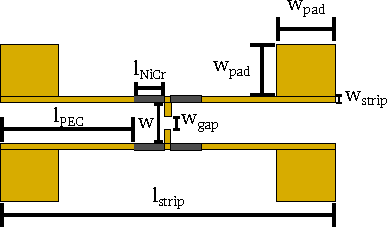
\includegraphics[width=\linewidth]{figures/sim_NICR_abmessungen.pdf}
        \label{fig:NICR}
    \end{subfigure}
    \hspace{0.1em}
    \begin{subtable}[c]{0.45\textwidth}
        \centering
        \begin{tabular}{ll}
        \toprule
        Variable & Length [$\mu m$]\\
        \midrule
        l\textsubscript{strip} & 1900 \\
        w\textsubscript{gap} & 5 \\
        w & 15 \\
        w\textsubscript{strip} & 5 \\
        w\textsubscript{pad} & 200 \\
        l\textsubscript{NiCr} & var. \\
        l\textsubscript{PEC} & var. \\
        \bottomrule
        \end{tabular}
        \label{tab:table}
    \end{subtable}
    \caption{Important antenna dimensions used for simulation of H-Dipoles. l\textsubscript{NiCr} is set to zero when simulating the reference H-Dipole antenna.}
    \label{fig:sim_dimensions}
\end{figure}

\subsection{Design of NiCr-Modified Antennas}

To investigate the impact of incorporating resistive materials into the antenna feed, the reference H-Dipole topology is systematically modified by introducing NiCr strips into the feeding structure. For a meaningful comparison with the reference design, all other structural and simulation parameters are kept identical to those described previously.
NiCr is defined as an ohmic sheet material with a sheet resistance of \num{22} \si{\ohm/sq} in CST.

In the modified design, segments of the original perfectly electrically conducting (PEC) feeding lines are selectively replaced by NiCr. The integration of NiCr begins at the antenna’s electrodes, such that increasing the NiCr length moves the resistive section closer to the antenna’s contact pads. In CST, this is done by defining a length $l_{NiCr}$ that can be modified at will. Additionally, the length of the complete feeding strip $l_{strip}$ consists of the portion of the strip made up of PEC $l_{PEC}$ and the portion of the strip made up of the NiCr sheet $l_{NiCr}$. The values of $l_{PEC}$ and $l_{NiCr}$ always need to add up to $l_{strip}$, which is \num{1900} \si{\micro\meter} in this case. For efficient simulations where many possible values of $l_{NiCr}$ are to be evaluated, $l_{PEC}$ is defined as $l_{PEC} = l_{strip}/2 - l_{NiCr}$. This definition ensures that increasing the length of $l_{NiCr}$ automatically decreases the length of $l_{PEC}$, allowing the overall geometry of the feeding strip to remain constant across all configurations.


The resistance of the NiCr section is directly proportional to its length, as given by the relation: $R_{NiCr} \propto l_{NiCr}$. Thus, multiple configurations with varying strip lengths $l_{NiCr}$ are simulated in order to evaluate their impact on antenna performance and determine suitable parameters for future fabrication.

\subsection{Simulation Parameters}

Simulations are carried out using CST Studio Suite’s time-domain solver, which employs the finite integration technique (FIT) to solve Maxwell’s equations. A hexahedral mesh is used, and the simulation accuracy is set to \num{-30} \si{\decibel}. Field monitors are implemented at two distinct frequencies: \num{100} \si{\giga\hertz} and \num{1} \si{\tera\hertz}. At these frequencies, the electromagnetic field distribution is recorded. Monitors for the electric field, magnetic field, and surface current are used to analyze the antenna's radiation characteristics and internal behavior.
